\documentclass[a4paper, 10pt, twoside]{article}
\usepackage[left=2cm, right=2cm, top=2cm, bottom=3cm]{geometry}
\usepackage{amsmath}
\usepackage[shortlabels]{enumitem}
\usepackage{bbold}
\usepackage{cases}
\usepackage{systeme}
\usepackage{graphicx}
\usepackage{bm}
\usepackage{float}

\begin{document}

\title{Machine Learning - Theoretical exercise 5}
\author{T\'eo Bouvard}
\maketitle

\section*{Problem 1}
Let $\varphi$ be a linear function used as the activation function for the two-layer network. As $\varphi$ is linear, we have $\varphi(u) = ku$, with $k \in \mathbb{R}$.
We first compute the outputs at the first layer.

\begin{align*}
    \bm{y}^{(1)} &= \varphi(\bm{\Theta}^{(1)}\bm{x}) \\
    &= k\bm{\Theta}^{(1)}\bm{x}
\end{align*}

We can now use this result for computing the outputs at the second layer.

\begin{align*}
    \bm{y}^{(2)} &= \varphi(\bm{\Theta}^{(2)}\bm{y}^{(1)}) \\
    &= \varphi(\bm{\Theta}^{(2)}k\bm{\Theta}^{(1)}\bm{x}) \\
    &= k^2\bm{\Theta}^{(2)}\bm{\Theta}^{(1)}\bm{x}
\end{align*}

We see that this result is equivalent to a single layer network having $k^2\bm{\Theta}^{(2)}\bm{\Theta}^{(1)}$ as its weight matrix and constant activation function.

\section*{Problem 2}

\begin{enumerate}[a)]
	\item The network has the following structure.
	\begin{figure}[h]
        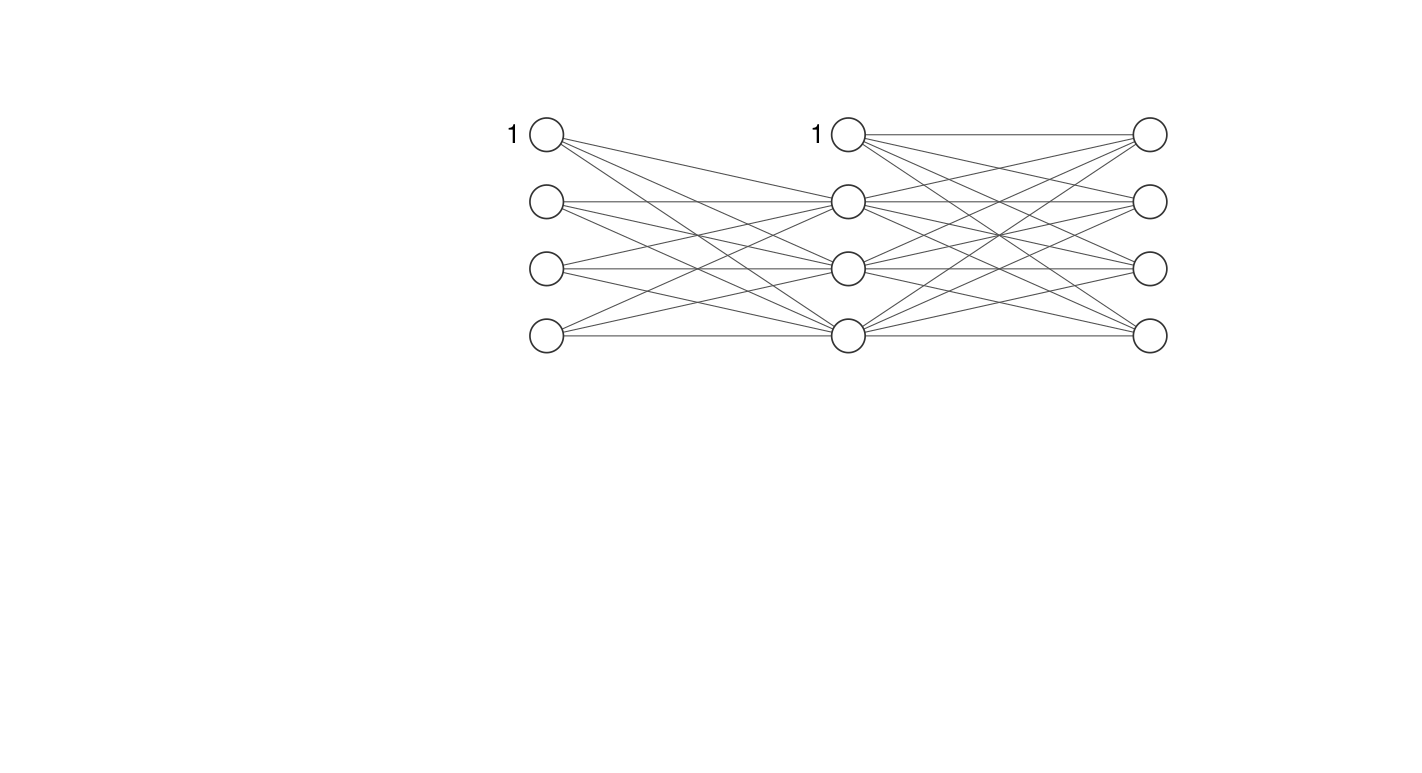
\includegraphics[width=0.8 \textwidth]{nn.png}
    \end{figure}

    \item Normalizing the training vectors gives us the following normalized dataset.
    
    \begin{align*}
        x_1 = \begin{bmatrix}1 \\ \frac{1}{4} \\ \frac{1}{4}\end{bmatrix}
        x_2 = \begin{bmatrix}1 \\ \frac{1}{4} \\ 0\end{bmatrix}
        x_3 = \begin{bmatrix}\frac{1}{2} \\ 0 \\ \frac{1}{4}\end{bmatrix}
        x_4 = \begin{bmatrix}\frac{1}{2} \\ 0 \\ 0\end{bmatrix}
    \end{align*}

    \item 
    Let $\sigma$ be the sigmoid function used as activation function for the network. We could compute the consecutive outputs by performing a matrix multiplication and then a matrix addition.

    \[
        \bm{y} = \sigma(\bm{\Theta}\bm{x} + b)
    \]

    but it is easier to incorporate the bias to our weight matrix, and add a unit component to each of our training vector, as this allows us to perform a single matrix multiplication. In the following, we this augmented weight matrix will be denoted $\bm{\Theta}$.

    We first compute the output at the first hidden layer.
    
    \begin{align*}
        \bm{y}^{(1)} &= \sigma(\bm{\Theta}^{(1)}\bm{x}) \\
    \end{align*}

\end{enumerate}


\end{document}
